\chapter{Inheritance: Reusing Code the Smart Way}

\section{Introduction: Real-Life Hook}

Rana notices something interesting:
\begin{itemize}
    \item He has his father’s height
    \item He has his mother’s smile
    \item He learned many habits from his family
\end{itemize}

In real life, children \textbf{inherit features from parents}.

In programming, classes can also inherit:
\begin{itemize}
    \item Data
    \item Methods
\end{itemize}

This powerful idea is called \textbf{Inheritance}.

\section{Concept: What Is Inheritance?}

\begin{definition}{Inheritance}
Inheritance is an OOP concept where a \textbf{new class (child) uses properties and methods of an existing class (parent)}.
\end{definition}

Inheritance helps:
\begin{itemize}
    \item Reuse code
    \item Reduce duplication
    \item Organize programs logically
\end{itemize}

\section{Parent and Child Classes}

\begin{itemize}
    \item Parent class $\rightarrow$ base class
    \item Child class $\rightarrow$ derived class
\end{itemize}

Example:

\begin{verbatim}
class Person:
    def speak(self):
        print("Person can speak")
\end{verbatim}

\begin{verbatim}
class Student(Person):
    def study(self):
        print("Student studies")
\end{verbatim}

\section{Using Inherited Methods}

\begin{verbatim}
s = Student()
s.speak()
s.study()
\end{verbatim}

The \texttt{Student} class:
\begin{itemize}
    \item Inherits \texttt{speak()} from \texttt{Person}
    \item Has its own method \texttt{study()}
\end{itemize}

\section{Inheritance with Constructor}

\begin{verbatim}
class Person:
    def __init__(self, name):
        self.name = name

class Student(Person):
    def __init__(self, name, roll):
        super().__init__(name)
        self.roll = roll
\end{verbatim}

\begin{itemize}
    \item \texttt{super()} calls parent constructor
    \item Avoids rewriting parent initialization
\end{itemize}

\section{Mini-Project: School Members System}

\textbf{Goal:} Model school members using inheritance.

\begin{verbatim}
class Person:
    def __init__(self, name):
        self.name = name

    def display(self):
        print("Name:", self.name)

class Student(Person):
    def __init__(self, name, roll):
        super().__init__(name)
        self.roll = roll

    def display(self):
        super().display()
        print("Roll:", self.roll)

class Teacher(Person):
    def __init__(self, name, subject):
        super().__init__(name)
        self.subject = subject

    def display(self):
        super().display()
        print("Subject:", self.subject)

s = Student("Ayesha", 5)
t = Teacher("Mr. Karim", "Math")

s.display()
t.display()
\end{verbatim}

Students learn:
\begin{itemize}
    \item Parent-child relationships
    \item Method overriding
    \item Code reuse
\end{itemize}

\section{Diagram: Inheritance Hierarchy}

\begin{center}
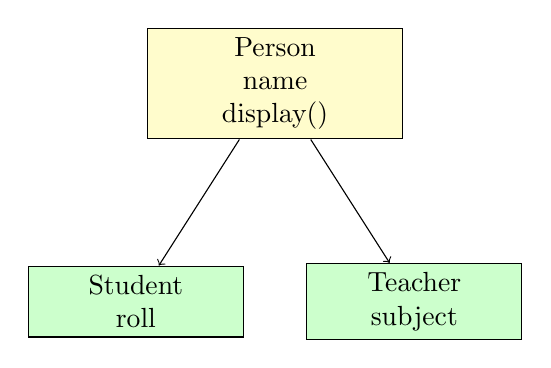
\begin{tikzpicture}[node distance=2.5cm]
\node (parent) [draw, rectangle, fill=yellow!20, text width=3cm, align=center] {Person\\
name\\
display()};
\node (child1) [draw, rectangle, fill=green!20, below left of=parent, yshift=-1cm, text width=2.5cm, align=center] {Student\\
roll};
\node (child2) [draw, rectangle, fill=green!20, below right of=parent, yshift=-1cm, text width=2.5cm, align=center] {Teacher\\
subject};

\draw[->] (parent) -- (child1);
\draw[->] (parent) -- (child2);
\end{tikzpicture}
\end{center}

\section{Types of Inheritance (Brief)}

\begin{itemize}
    \item Single inheritance
    \item Multiple inheritance (advanced)
    \item Multilevel inheritance
\end{itemize}

\textit{Note:} This book focuses mainly on \textbf{single inheritance} for beginners.

\section{Advantages of Inheritance}

\begin{itemize}
    \item Saves time
    \item Improves code clarity
    \item Makes maintenance easier
    \item Supports real-world modeling
\end{itemize}

\section{Key Concepts}

\begin{itemize}
    \item Inheritance allows code reuse
    \item Parent class passes features to child class
    \item \texttt{super()} accesses parent methods
    \item Method overriding customizes behavior
\end{itemize}

\section{End-of-Chapter Exercises}

\subsection{Very Short Questions}

\begin{enumerate}
    \item What is inheritance?
    \item What is a parent class?
    \item What does \texttt{super()} do?
\end{enumerate}

\subsection{Short Answer Questions}

\begin{enumerate}
    \item Explain inheritance using a real-life example.
    \item Write a simple parent and child class.
    \item Why is inheritance useful in large programs?
\end{enumerate}

\subsection{Activity-Based Exercises}

\begin{enumerate}
    \item Create a \texttt{Vehicle} class and inherit \texttt{Car} from it.
    \item Design a \texttt{Animal} parent class and \texttt{Dog} child class.
    \item Modify the school system to add a \texttt{Staff} class.
\end{enumerate}

\section{Teacher Notes}

\marginnote{
\textbf{Learning Objectives}
\begin{itemize}
    \item Students understand inheritance clearly
    \item Students use parent and child classes
    \item Students apply code reuse
\end{itemize}

\textbf{Teaching Tips}
\begin{itemize}
    \item Use family tree diagrams
    \item Emphasize ``is-a'' relationship
    \item Show reduction of repeated code
\end{itemize}

\textbf{Assessment}
\begin{itemize}
    \item Correct inheritance structure
    \item Proper use of \texttt{super()}
\end{itemize}
}